\documentclass{beamer}
\usepackage[utf8]{inputenc}
\usefonttheme{professionalfonts}
\usepackage{xcolor}
\usepackage{graphicx}
\usepackage{amsmath, amsthm, amssymb, amsfonts}
\usepackage{bbm}

\usepackage{tikz}
\usepackage{pgfplots}

\newcommand{\topline}{%
  \tikz[remember picture,overlay] {%
    \draw[gray, thick] ([xshift=1cm,yshift=-1.2cm]current page.north west)
             -- ([xshift=-1cm,yshift=-1.2cm,xshift=\paperwidth]current page.north west);}}

\usepackage{caption}
\usepackage{tabularx, booktabs}
\usepackage{multirow}
\usepackage{multicol}

\definecolor{light_red}{RGB}{209,105,81}
\definecolor{fair_red}{RGB}{237,27,47}
\definecolor{light_green}{RGB}{58,181,75}
\definecolor{thick_blue}{RGB}{5,43,108}
\definecolor{fair_blue}{RGB}{0,112,192}
\definecolor{light_blue}{RGB}{0,153,228}
\definecolor{light_brown}{RGB}{132, 60, 11}

\setbeamertemplate{frametitle}[default][center]
\setbeamertemplate{navigation symbols}{}
\setbeamerfont{footline}{series=\bfseries}
\setbeamertemplate{footline}[page number]

\setbeamertemplate{itemize items}[circle]
\setbeamercolor{itemize item}{fg=black}

\setbeamercolor{block title}{fg = black, bg = light_blue!40}
\setbeamercolor{block body}{fg = black, bg = white}
\setbeamertemplate{blocks}[rounded][shadow]
\setbeamercolor{block title example}{fg = black, bg = orange!40}
\setbeamercolor{block body example}{fg = black, bg = white}

\setbeamercolor{block title alerted}{fg = black, bg = light_red!40}
\setbeamercolor{section number projected}{bg=gray}
\setbeamercolor{section number projected}{bg=gray}
\setbeamercolor{subsection number projected}{bg=gray}

\setbeamertemplate{footline}[frame number]{}


\begin{document}

\begin{frame}[plain]

\begin{columns}
\begin{column}{0.5\textwidth}

\begin{center}
{\color{black!80}\Large\textbf{Deblurring Images}

\vspace{0.2em}

\large\textbf{Matrices, Spectra, and Filtering}}

\small

\vspace{2em}

\textbf{Xinyu Chen} ({\color{fair_blue}\url{https://xinychen.github.io}})

\vspace{0.8em}

{October 11, 2022}

\end{center}

\end{column}

\begin{column}{0.5\textwidth}

\begin{center}

\includegraphics[scale=0.12]{graphics/book-cover.png}
\end{center}

\end{column}
\end{columns}

\end{frame}

\begin{frame}[plain]

\large
\begin{itemize}
\item[\color{black}$\circ$] \textbf{Chapter 1: The Image Deblurring Problem}
\color{gray}
\item[\color{gray}$\circ$] \textbf{Chapter 4: Structured Matrix Computations}
\end{itemize}

\end{frame}

\begin{frame}{\color{black}\textbf{The Image Deblurring Problem}}
\topline

About the image deblurring\footnote{The images and Matlab functions discussed in the book are available at {\color{fair_blue}\url{https://archive.siam.org/books/fa03/}}.}:
\begin{itemize}\small
\item \textbf{[Significance]} Image deblurring is fundamental in making pictures sharp and useful.
\item \textbf{[General idea]} Recovering the original and sharp image by using a mathematical model of blurring process.
\item \textbf{[Fact]} No hope to recover the original image exactly!
\item \textbf{[Technical goal]} Develop efficient and reliable algorithms for recovering as much information as possible from the given data.
\item \textbf{[Representation]} A digital image is a two- or three-dimensional array of numbers representing intensities on a grayscale or color scale.
\end{itemize}
    
\end{frame}

\begin{frame}{\color{black}\textbf{The Image Deblurring Problem}}
\topline

A blurred picture and simple linear model.
\small
\begin{itemize}
\item \textbf{Sharp image} vs. \textbf{blurred image}
\begin{center}
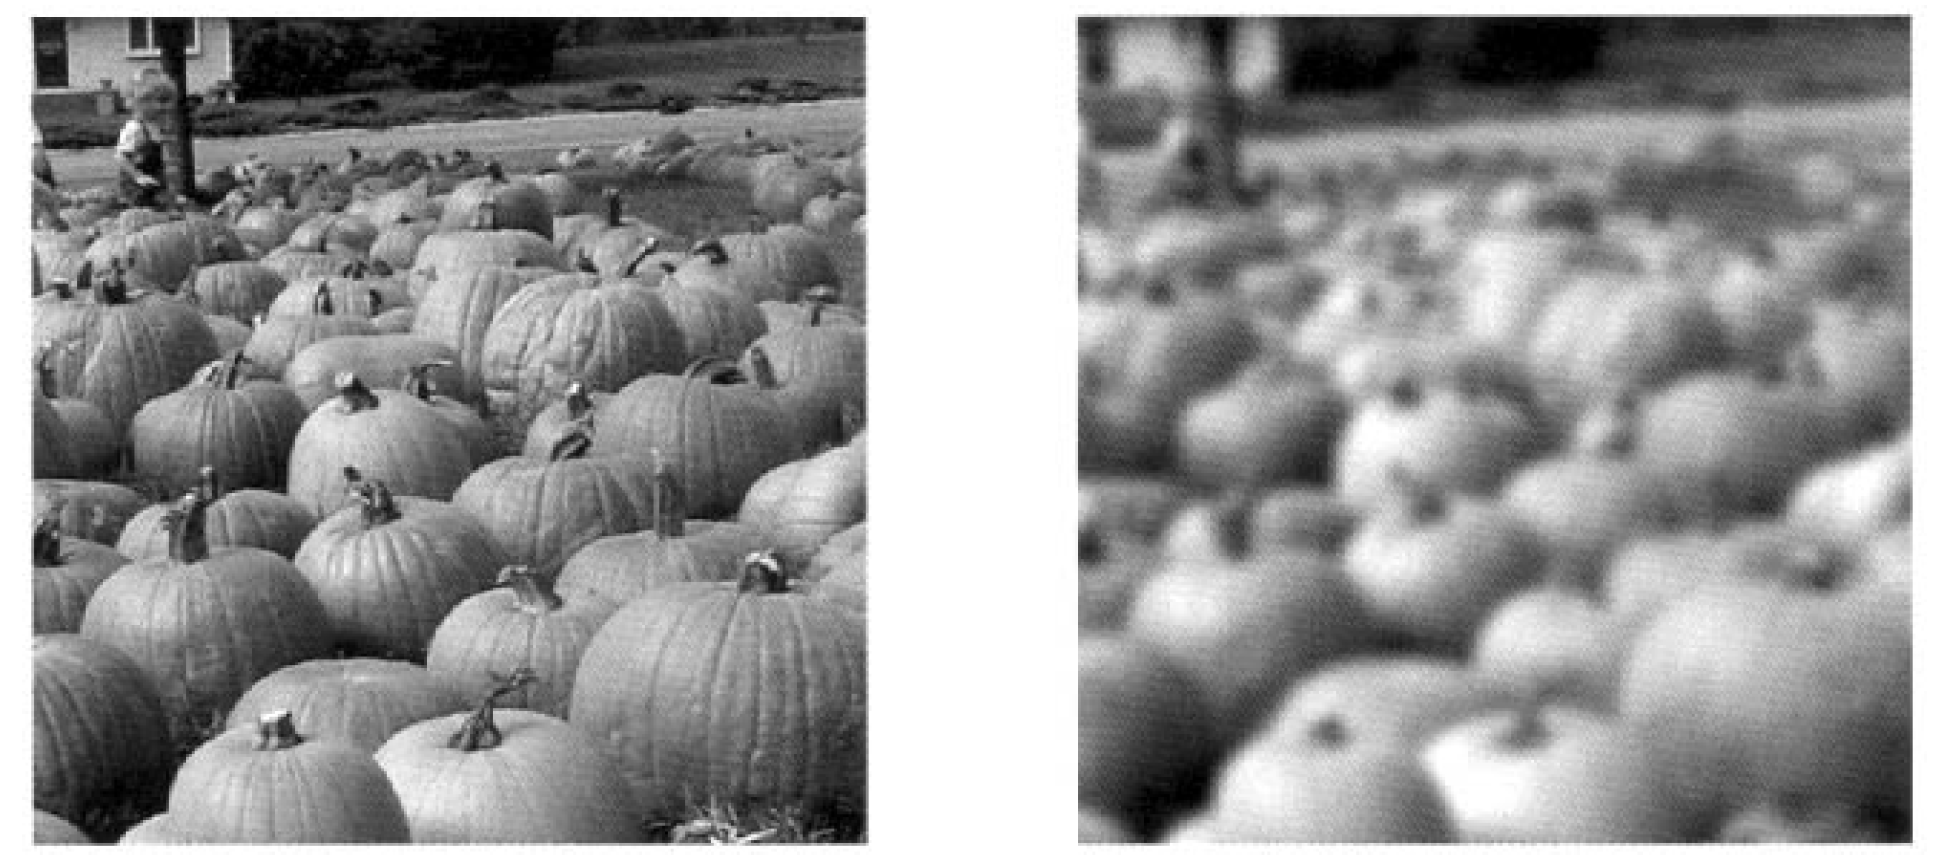
\includegraphics[width=0.75\textwidth]{graphics/sharp-vs-blurred-images.png}
\end{center}
\item Notation: $\boldsymbol{X}\in\mathbb{R}^{m\times n}$ (desired \textbf{sharp} image) vs. $\boldsymbol{B}\in\mathbb{R}^{m\times n}$ (recorded \textbf{blurred} image)
\item A simple linear model:
\begin{itemize}\footnotesize
    \item[\color{black}$\circ$] Suppose the blurring of the columns in the image is independent of the blurring of the rows.
    \item[\color{black}$\circ$] \textbf{Bilinear relationship}: $\boxed{\boldsymbol{A}_{c}\boldsymbol{X}\boldsymbol{A}_{r}^\top=\boldsymbol{B}}$
\end{itemize}
\end{itemize}

\end{frame}

\begin{frame}{\color{black}\textbf{The Image Deblurring Problem}}
\topline

A first attempt at deblurring.
\small
\begin{itemize}
\item Recall that the simple linear model:
\begin{equation}
\boldsymbol{A}_{c}\boldsymbol{X}\boldsymbol{A}_{r}^\top=\boldsymbol{B}\quad\Longrightarrow\quad\boldsymbol{X}_{\text{naive}}=\boldsymbol{A}_{c}^{-1}\boldsymbol{B}(\boldsymbol{A}_{r}^{\top})^{-1}
\end{equation}
ignores several types of errors.
\item Let 
\begin{equation}
\boldsymbol{B}_{\text{exact}}=\boldsymbol{A}_{c}\boldsymbol{X}\boldsymbol{A}_{r}^\top
\end{equation}
be the ideal (noise-free) blurred image, ignoring all kinds of errors.
\item Consider small random errors (noise) in the recorded blurred image:
\begin{equation}
\boldsymbol{B}=\boldsymbol{B}_{\text{exact}}+\boldsymbol{E}=\boldsymbol{A}_{c}\boldsymbol{X}\boldsymbol{A}_{r}^\top+\boldsymbol{E}
\end{equation}
where $\boldsymbol{E}\in\mathbb{R}^{m\times n}$ is the \textbf{noise image}.
\end{itemize}

\end{frame}

\begin{frame}{\color{black}\textbf{The Image Deblurring Problem}}
\topline

A first attempt at deblurring.
\small

\begin{exampleblock}{\footnotesize\textbf{The naive reconstruction}}
Recall that
\begin{equation}
\begin{cases}
\boldsymbol{X}_{\text{naive}}=\boldsymbol{A}_{c}^{-1}\boldsymbol{B}(\boldsymbol{A}_{r}^\top)^{-1} \\
\boldsymbol{B}=\boldsymbol{B}_{\text{exact}}+\boldsymbol{E}=\boldsymbol{A}_{c}\boldsymbol{X}\boldsymbol{A}_{r}^\top+\boldsymbol{E}
\end{cases}
\end{equation}
we therefore have the naive reconstruction:
\begin{equation}
\begin{aligned}
\boldsymbol{X}_{\text{naive}}=&\boldsymbol{A}_{c}^{-1}\boldsymbol{B}(\boldsymbol{A}_{r}^{\top})^{-1} \\
=&\boldsymbol{A}_{c}^{-1}\boldsymbol{B}_{\text{exact}}(\boldsymbol{A}_{r}^{\top})^{-1}+\boldsymbol{A}_{c}^{-1}\boldsymbol{E}(\boldsymbol{A}_{r}^{\top})^{-1} \\
=&\boldsymbol{X}+\boldsymbol{A}_{c}^{-1}\boldsymbol{E}(\boldsymbol{A}_{r}^{\top})^{-1}
\end{aligned}
\end{equation}

\end{exampleblock}

\begin{itemize}
    \item The blurred image consists of two components: the first component is the \textbf{exact image}, and the second component is the \textbf{inverted noise}.
\end{itemize}

\end{frame}

\begin{frame}{\color{black}\textbf{The Image Deblurring Problem}}
\topline

A first attempt at deblurring.
\small
\begin{itemize}
\item A simple test: \textbf{Exact image} $\boldsymbol{X}\in\mathbb{R}^{m\times n}$ vs. \textbf{blurred image} $\boldsymbol{B}\in\mathbb{R}^{m\times n}$
\begin{center}
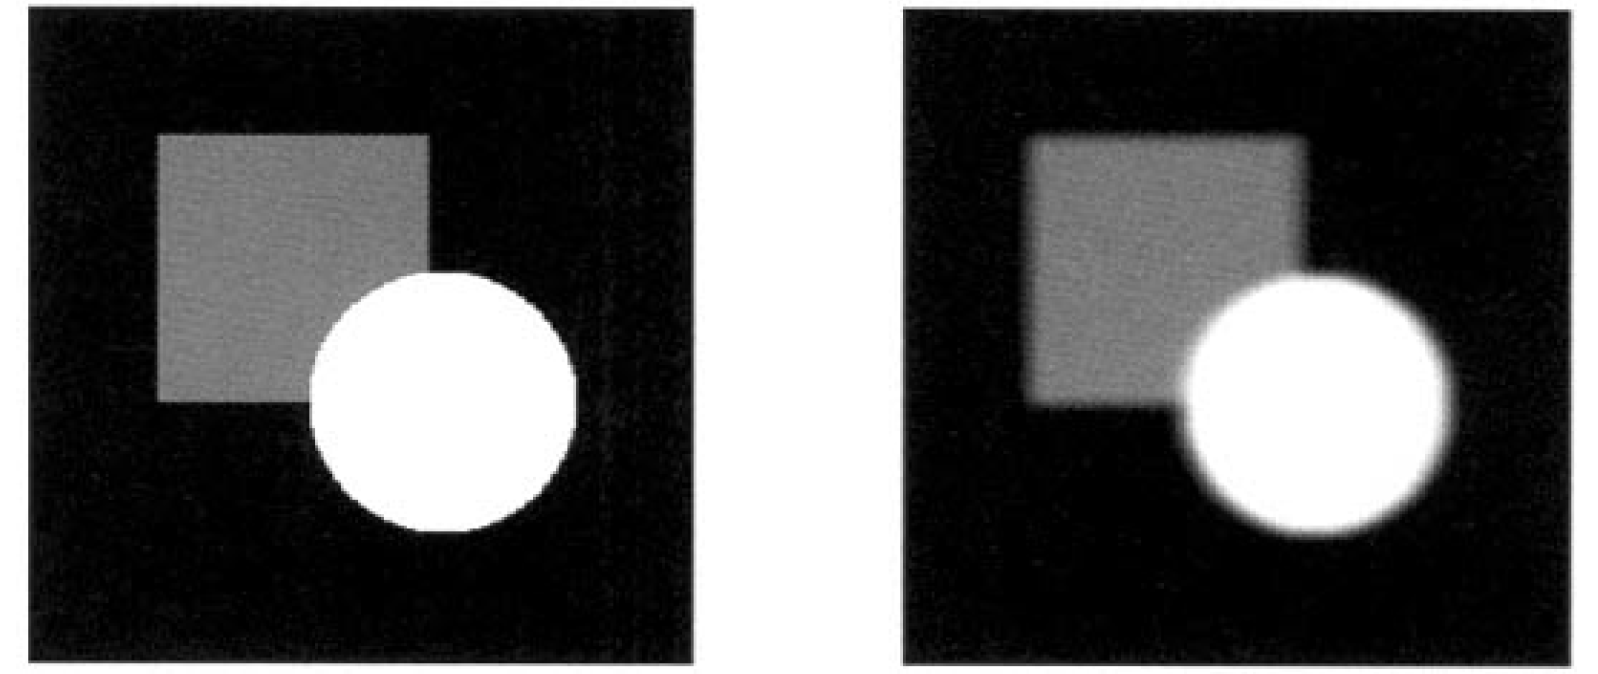
\includegraphics[width=0.75\textwidth]{graphics/exact-vs-blurred-images.png}
\end{center}
\end{itemize}
    
\end{frame}

\begin{frame}{\color{black}\textbf{The Image Deblurring Problem}}
\topline
\small
\begin{alertblock}{\footnotesize\textbf{Lemma}}
For the simple model $\boldsymbol{B}=\boldsymbol{A}_{c}\boldsymbol{X}\boldsymbol{A}_{r}^\top+\boldsymbol{E}$, the relative error in the naive reconstruction $\boldsymbol{X}_{\text{naive}}=\boldsymbol{A}_{c}^{-1}\boldsymbol{B}(\boldsymbol{A}_{r}^\top)^{-1}$ satisfies
\begin{equation}
\frac{\|\boldsymbol{X}_{\text{naive}}-\boldsymbol{X}\|_{F}}{\|\boldsymbol{X}\|_{F}}\leq \text{cond}(\boldsymbol{A}_{c})\cdot\text{cond}(\boldsymbol{A}_{r})\cdot\frac{\|\boldsymbol{E}\|_{F}}{\|\boldsymbol{B}\|_{F}}
\end{equation}
where $\|\cdot\|_{F}$ denotes the Frobenius norm\footnote{For any $\boldsymbol{X}\in\mathbb{R}^{m\times n}$, we have $\|\boldsymbol{X}\|_{F}=\sqrt{\sum_{i=1}^{m}\sum_{j=1}^{n}x_{ij}^2}$.}, and $\text{cond}(\cdot)$ denotes the conditional number\footnote{For any $\boldsymbol{A}\in\mathbb{R}^{N\times N}$ whose singular values are strictly positive, namely, $\sigma_1\geq\cdots\geq\sigma_N>0$, we have $\text{cond}(\boldsymbol{A})=\sigma_1/\sigma_N$.}.
\end{alertblock}
    
\end{frame}

\begin{frame}{\color{black}\textbf{The Image Deblurring Problem}}
\topline

Deblurring using a general linear model.
\begin{itemize}\small
\item In most situations, the blur is indeed \textbf{linear}, or at least well approximated by a linear model.
\item A general linear model via \textbf{vectorization}.
\begin{itemize}\footnotesize
    \item[\color{black}$\circ$] Given sharp image $\boldsymbol{X}\in\mathbb{R}^{m\times n}$ and blurred image $\boldsymbol{B}\in\mathbb{R}^{m\times n}$, since the blurring is assumed to be a linear operation, there must exist a large \textbf{blurring matrix} $\boldsymbol{A}\in\mathbb{R}^{N\times N}$ ($N=mn$) such that
    \begin{equation}
    \boldsymbol{A}\boldsymbol{x}=\boldsymbol{b}
    \end{equation}
    with
    \begin{equation}
    \boldsymbol{x}=\text{vec}(\boldsymbol{X})=\begin{bmatrix} \boldsymbol{x}_{1} \\ \vdots \\ \boldsymbol{x}_{n} \end{bmatrix}\in\mathbb{R}^{N},\quad\boldsymbol{b}=\text{vec}(\boldsymbol{B})=\begin{bmatrix} 
    \boldsymbol{b}_{1} \\ \vdots \\ \boldsymbol{b}_{n} \end{bmatrix}\in\mathbb{R}^{N}
    \end{equation}
    \item[\color{black}$\circ$] The naive approach to image deblurring is simply to solve this linear algebraic system.
\end{itemize}
\end{itemize}

\end{frame}

\begin{frame}{\color{black}\textbf{The Image Deblurring Problem}}
\topline

Deblurring using a general linear model.
\small
\begin{exampleblock}{\footnotesize\textbf{The naive reconstruction (matrix-form)}}
Recall that
\begin{equation}
\begin{cases}
\boldsymbol{X}_{\text{naive}}=\boldsymbol{A}_{c}^{-1}\boldsymbol{B}(\boldsymbol{A}_{r}^\top)^{-1} \\
\boldsymbol{B}=\boldsymbol{B}_{\text{exact}}+\boldsymbol{E}=\boldsymbol{A}_{c}\boldsymbol{X}\boldsymbol{A}_{r}^\top+\boldsymbol{E}
\end{cases}
\end{equation}
we therefore have the naive reconstruction:
\begin{equation}
\begin{aligned}
\boldsymbol{X}_{\text{naive}}=&\boldsymbol{A}_{c}^{-1}\boldsymbol{B}(\boldsymbol{A}_{r}^{\top})^{-1} \\
=&\boldsymbol{A}_{c}^{-1}\boldsymbol{B}_{\text{exact}}(\boldsymbol{A}_{r}^{\top})^{-1}+\boldsymbol{A}_{c}^{-1}\boldsymbol{E}(\boldsymbol{A}_{r}^{\top})^{-1} \\
=&\boldsymbol{X}+\boldsymbol{A}_{c}^{-1}\boldsymbol{E}(\boldsymbol{A}_{r}^{\top})^{-1}
\end{aligned}
\end{equation}

\end{exampleblock}

\begin{exampleblock}{\footnotesize\textbf{The naive reconstruction (vector-form)}}
Vectorize blurred image $\boldsymbol{B}$ and noise image $\boldsymbol{E}$ as $\boldsymbol{b}_{\text{exact}}=\text{vec}(\boldsymbol{B}_{\text{exact}})=\boldsymbol{A}\boldsymbol{x}$ and $\boldsymbol{e}=\text{vec}(\boldsymbol{E})$, respectively, then we have
\begin{equation}
\boldsymbol{x}_{\text{naive}}=\boldsymbol{A}^{-1}\boldsymbol{b}=\boldsymbol{A}^{-1}\boldsymbol{b}_{\text{exact}}+\boldsymbol{A}^{-1}\boldsymbol{e}=\boldsymbol{x}+\boldsymbol{A}^{-1}\boldsymbol{e}
\end{equation}
\end{exampleblock}

\end{frame}

\begin{frame}{\color{black}\textbf{The Image Deblurring Problem}}
\topline

Deblurring using a general linear model.

\small
\begin{itemize}
\item Relationship between matrix- and vector-form reconstruction:
\begin{equation}
\begin{aligned}
\boldsymbol{X}_{\text{naive}}&=\boldsymbol{A}_{c}^{-1}\boldsymbol{B}(\boldsymbol{A}_{r}^{\top})^{-1} \\
\Longrightarrow~\boldsymbol{x}_{\text{naive}}&=(\boldsymbol{A}_{r}^{-1}\otimes\boldsymbol{A}_{c}^{-1})\boldsymbol{b} \\
&=(\boldsymbol{A}_{r}\otimes\boldsymbol{A}_{c})^{-1}\boldsymbol{b}
\end{aligned}
\end{equation}
it therefore demonstrates that $\boldsymbol{A}\triangleq\boldsymbol{A}_{r}\otimes\boldsymbol{A}_{c}$.
\item Property of Kronecker product $\otimes$:
\begin{alertblock}{\footnotesize\textbf{Proposition}}
Let $\boldsymbol{A}\in\mathbb{R}^{m\times m}$, $\boldsymbol{X}\in\mathbb{R}^{m\times n}$, and $\boldsymbol{B}\in\mathbb{R}^{n\times n}$ be three matrices commensurate from multiplication in that order, then it holds that
\begin{equation}
\text{vec}(\boldsymbol{A}\boldsymbol{X}\boldsymbol{B})=(\boldsymbol{B}^\top\otimes\boldsymbol{A})\text{vec}(\boldsymbol{X})
\end{equation}
\end{alertblock}

\end{itemize}

\end{frame}

\begin{frame}{\color{black}\textbf{The Image Deblurring Problem}}
\topline

Deblurring using a general linear model.

\small
\begin{alertblock}{\footnotesize\textbf{Singular value decomposition (SVD)}}
For any $\boldsymbol{A}\in\mathbb{R}^{N\times N}$ whose singular values are strictly positive, we have
\begin{equation}
\boldsymbol{A}=\boldsymbol{U}\boldsymbol{\Sigma}\boldsymbol{V}^\top=\sum_{i=1}^{N}\sigma_{i}\boldsymbol{u}_{i}\boldsymbol{v}_{i}^\top\quad\Longrightarrow\quad\boldsymbol{A}^{-1}=\sum_{i=1}^{N}\frac{1}{\sigma_{i}}\boldsymbol{u}_{i}\boldsymbol{v}_{i}^\top
\end{equation}
\end{alertblock}

\begin{exampleblock}{\footnotesize\textbf{The naive reconstruction with SVD}}
The naive reconstruction can be written as follows,
\begin{equation}
\boldsymbol{x}_{\text{naive}}=\boldsymbol{A}^{-1}\boldsymbol{b}=\boldsymbol{V}\boldsymbol{\Sigma}^{-1}\boldsymbol{U}^\top\boldsymbol{b}=\sum_{i=1}^{N}\frac{\boldsymbol{u}_{i}^\top\boldsymbol{b}}{\sigma_i}\boldsymbol{v}_{i}
\end{equation}
in which the inverted noise is
\begin{equation}
\boldsymbol{A}^{-1}\boldsymbol{e}=\boldsymbol{V}\boldsymbol{\Sigma}^{-1}\boldsymbol{U}^\top\boldsymbol{e}=\sum_{i=1}^{N}\frac{\boldsymbol{u}_{i}^\top\boldsymbol{e}}{\sigma_i}\boldsymbol{v}_{i}
\end{equation}
\end{exampleblock}

\end{frame}

\begin{frame}{\color{black}\textbf{The Image Deblurring Problem}}
\topline

Deblurring using a general linear model.

\small

\begin{itemize}
\item Recall that the inverted noise is
\begin{equation*}
\boldsymbol{A}^{-1}\boldsymbol{e}=\boldsymbol{V}\boldsymbol{\Sigma}^{-1}\boldsymbol{U}^\top\boldsymbol{e}=\sum_{i=1}^{N}\frac{\boldsymbol{u}_{i}^\top\boldsymbol{e}}{\sigma_i}\boldsymbol{v}_{i}
\end{equation*}
\item Properties for image deblurring problems:
\begin{itemize}\footnotesize
    \item[\color{black}$\circ$] The error components $|\boldsymbol{u}_{i}^\top\boldsymbol{e}|$ are small and typically of roughly the same order of magnitude for all $i$.
    \item[\color{black}$\circ$] The singular values decay to a value very close to zero. As a consequence, the condition number $\text{cond}(\boldsymbol{A})=\sigma_1/\sigma_N$ is very large, indicating that \textbf{the solution is very sensitive to perturbation and rounding errors}.
    \item[\color{black}$\circ$] \textbf{The singular vectors corresponding to the smaller singular values typically represent high-frequency information}. That is, as $i$ increases, the vectors $\boldsymbol{u}_{i}$ and $\boldsymbol{v}_{i}$ tend to have more sign changes.
\end{itemize}
\end{itemize}

\end{frame}

\begin{frame}{\color{black}\textbf{The Image Deblurring Problem}}
\topline

Deblurring using a general linear model.

\small

\begin{itemize}
\item Recall that the inverted noise is
\begin{equation*}
\boldsymbol{A}^{-1}\boldsymbol{e}=\boldsymbol{V}\boldsymbol{\Sigma}^{-1}\boldsymbol{U}^\top\boldsymbol{e}=\sum_{i=1}^{N}\frac{\boldsymbol{u}_{i}^\top\boldsymbol{e}}{\sigma_i}\boldsymbol{v}_{i}
\end{equation*}
\end{itemize}

\begin{exampleblock}{\footnotesize\textbf{Remark}}
For $\boldsymbol{A}^{-1}\boldsymbol{e}$, the quantities $\boldsymbol{u}_{i}^\top\boldsymbol{e}/\sigma_i$ are the expansion coefficients for the basis vectors $\boldsymbol{v}_{i}$. When these quantities are small in magnitude, the solution has very little contribution from $\boldsymbol{v}_{i}$, but when we divide by a small singular values such as $\sigma_N$, we greatly magnify the corresponding error component $\boldsymbol{u}_{N}^\top\boldsymbol{e}$ which in turn contributes a large multiple of the high-frequency information contained in $\boldsymbol{v}_{N}$ to the reconstruction solution.
\end{exampleblock}

\begin{itemize}
    \item Thus, we can remove the high-frequency components that are dominated by error.
\end{itemize}
\end{frame}

\begin{frame}{\color{black}\textbf{The Image Deblurring Problem}}
\topline

Deblurring using a general linear model.
\small
\begin{itemize}
\item The naive reconstruction with SVD:
\begin{equation}
\boldsymbol{x}_{\text{naive}}=\sum_{i=1}^{N}\frac{\boldsymbol{u}_{i}^\top\boldsymbol{b}}{\sigma_i}\boldsymbol{v}_{i}
\end{equation}
\item The truncated expansion with $k<N,k\in\mathbb{N}^{+}$:
\begin{equation}
\boldsymbol{x}_{k}=\sum_{i=1}^{k}\frac{\boldsymbol{u}_{i}^\top\boldsymbol{b}}{\sigma_i}\boldsymbol{v}_{i}
\end{equation}
which is indeed a reduced-rank linear model.
\item We may wonder if a different value for $k$ will produce a better reconstruction!
\end{itemize}

\end{frame}

\begin{frame}{\color{black}\textbf{Structured Matrix Computations}}
\topline

\small
\begin{itemize}
\item A general linear model:
\begin{equation}
\boldsymbol{b}=\boldsymbol{A}\boldsymbol{x}+\boldsymbol{e}
\end{equation}
with 
\begin{equation*}
\begin{cases}
\boldsymbol{b}=\text{vec}(\boldsymbol{B})\in\mathbb{R}^{N}\quad\text{(blurred image)} \\
\boldsymbol{x}=\text{vec}(\boldsymbol{X})\in\mathbb{R}^{N}\quad\text{(sharp image)} \\
\boldsymbol{e}=\text{vec}(\boldsymbol{E})\in\mathbb{R}^{N}~\quad\text{(noise image)} \\
\boldsymbol{A}\in\mathbb{R}^{N\times N}\quad\quad\quad\quad\text{(blurring matrix)}
\end{cases}
\end{equation*}
\item The deblurring algorithms use certain orthogonal or unitary decompositions of $\boldsymbol{A}$.
\begin{itemize}\footnotesize
    \item[\color{black}$\circ$] SVD: $\boldsymbol{A}=\boldsymbol{U}\boldsymbol{\Sigma}\boldsymbol{V}^\top$ vs. spectral decomposition\footnote{\footnotesize A matrix is unitary if $\tilde{\boldsymbol{U}}^{H}\tilde{\boldsymbol{U}}=\tilde{\boldsymbol{U}}\tilde{\boldsymbol{U}}^{H}=\boldsymbol{I}$ where $\tilde{\boldsymbol{U}}^{H}=\text{conj}(\tilde{\boldsymbol{U}})^\top$ is the complex conjugate transpose of $\tilde{\boldsymbol{U}}$. $\boldsymbol{\Lambda}$ is a diagonal matrix containing the eigenvalues of $\boldsymbol{A}$.}: $\boldsymbol{A}=\tilde{\boldsymbol{U}}\boldsymbol{\Lambda}\tilde{\boldsymbol{U}}^{H}$
    \item[\color{black}$\circ$] If $\boldsymbol{A}$ has real entries, then the elements in the matrices of the SVD will be real, but the entries in the spectral decomposition may be complex.
\end{itemize}
\end{itemize}
\end{frame}

\begin{frame}{\color{black}\textbf{Structured Matrix Computations}}
\topline

Basic structures.
\small

\begin{itemize}
\item Convolution is a mathematical operation.
\item If $p(s)$ and $x(s)$ are \textbf{continuous} functions, then the convolution of $p(s)$ and $x(s)$ is a function $b(s)$ having the form
\begin{equation}
b(s)=\int_{-\infty}^{\infty}p(s-t)x(t)dt
\end{equation}
each values of $b(s)$ is essentially a weighted average of the values of $x(s)$, where the weights are given by $p(s)$.
\item The \textbf{discrete} version of convolution is a summation over a finite number of terms.
\end{itemize}

\end{frame}

\end{document}
